\subsection{RGB-D Vision}

\label{sec:join-point-cloud}

Finally, we demonstrate an example of RGB-D vision. The convenience of the RGB-D camera is that the pixel depth information can be obtained physically. If the camera's internal and external parameters are known, we can calculate the position of any pixel in the world coordinate system to create a point cloud map. Now let's demonstrate it.

We have prepared 5 pairs of images in the slambook/ch5/rgbd folder. There are 5 RGB images from 1.png to 5.png under color/, and 5 corresponding depth maps under depth/. At the same time, the pose.txt file gives the camera's external position pose (in the form of $\bm{T}_\mathrm{wc}$) for five images. The pose record is in the same form as before, adding a rotating quaternion to the translation vector:
\[
[x,y,z,q_x,q_y,q_z,q_w],
\]
Where $q_w$ is the real part of the quaternion. For example, the external parameters of the first pair of graphs are:
\[
[-0.228993, 0.00645704, 0.0287837, -0.0004327, -0.113131, -0.0326832, 0.993042].
\]

Below we write a program to complete two things: (1). Calculate a point cloud corresponding to a pair of RGB-D images according to the internal parameters; (2). According to the camera pose of each picture (that is, the external parameter), put the point Clouds add up to form a map.

\begin{lstlisting}[language=C++,caption=slambook/ch5/rgbd/jointMap.cpp(part)]
Int main(int argc, char **argv) {
Vector<cv::Mat> colorImgs, depthImgs; // color and depth map
TrajectoryType poses; // camera pose

Ifstream fin("./pose.txt");
If (!fin) {
Cerr << "Please run this program in the directory with pose.txt" << endl;
Return 1;
}

For (int i = 0; i < 5; i++) {
Boost::format fmt("./%s/%d.%s"); //Image file format
colorImgs.push_back(cv::imread((fmt % "color" % (i + 1) % "png").str()));
depthImgs.push_back(cv::imread((fmt % "depth" % (i + 1) % "pgm").str(), -1)); // Read the original image with -1

Double data[7] = {0};
For (auto &d:data) fin >> d;
Sophus::SE3d pose(Eigen::Quaterniond(data[6], data[3], data[4], data[5]),
Eigen::Vector3d(data[0], data[1], data[2]));
Poses.push_back(pose);
}

/ / Calculate the point cloud and splicing
// camera internal reference 
Double cx = 325.5;
Double cy = 253.5;
Double fx = 518.0;
Double fy = 519.0;
Double depthScale = 1000.0;
Vector<Vector6d, Eigen::aligned_allocator<Vector6d>> pointcloud;
Pointcloud.reserve(1000000);

For (int i = 0; i < 5; i++) {
Cout << "Converted image: " << i + 1 << endl;
Cv::Mat color = colorImgs[i];
Cv::Mat depth = depthImgs[i];
Sophus::SE3d T = poses[i];
For (int v = 0; v < color.rows; v++)
For (int u = 0; u < color.cols; u++) {
Unsigned int d = depth.ptr<unsigned short>(v)[u]; // depth value
If (d == 0) continue; // 0 means no measurement
Eigen::Vector3d point;
Point[2] = double(d) / depthScale;
Point[0] = (u - cx) * point[2] / fx;
Point[1] = (v - cy) * point[2] / fy;
Eigen::Vector3d pointWorld = T * point;

Vector6d p;
P.head<3>() = pointWorld;
p[5] = color.data[v * color.step + u * color.channels()]; // blue
p[4] = color.data[v * color.step + u * color.channels() + 1]; // green
p[3] = color.data[v * color.step + u * color.channels() + 2]; // red
Pointcloud.push_back(p);
}
}

Cout << "point cloud total" << pointcloud.size() << "points." << endl;
showPointCloud(pointcloud);
Return 0;
}
\end{lstlisting}

After running the program, you can see the stitched point cloud map in the Pangolin window (see \autoref{fig:pointcloudmapping}). You can drag and drop to view.

\begin{figure}[!htp]
	\centering
	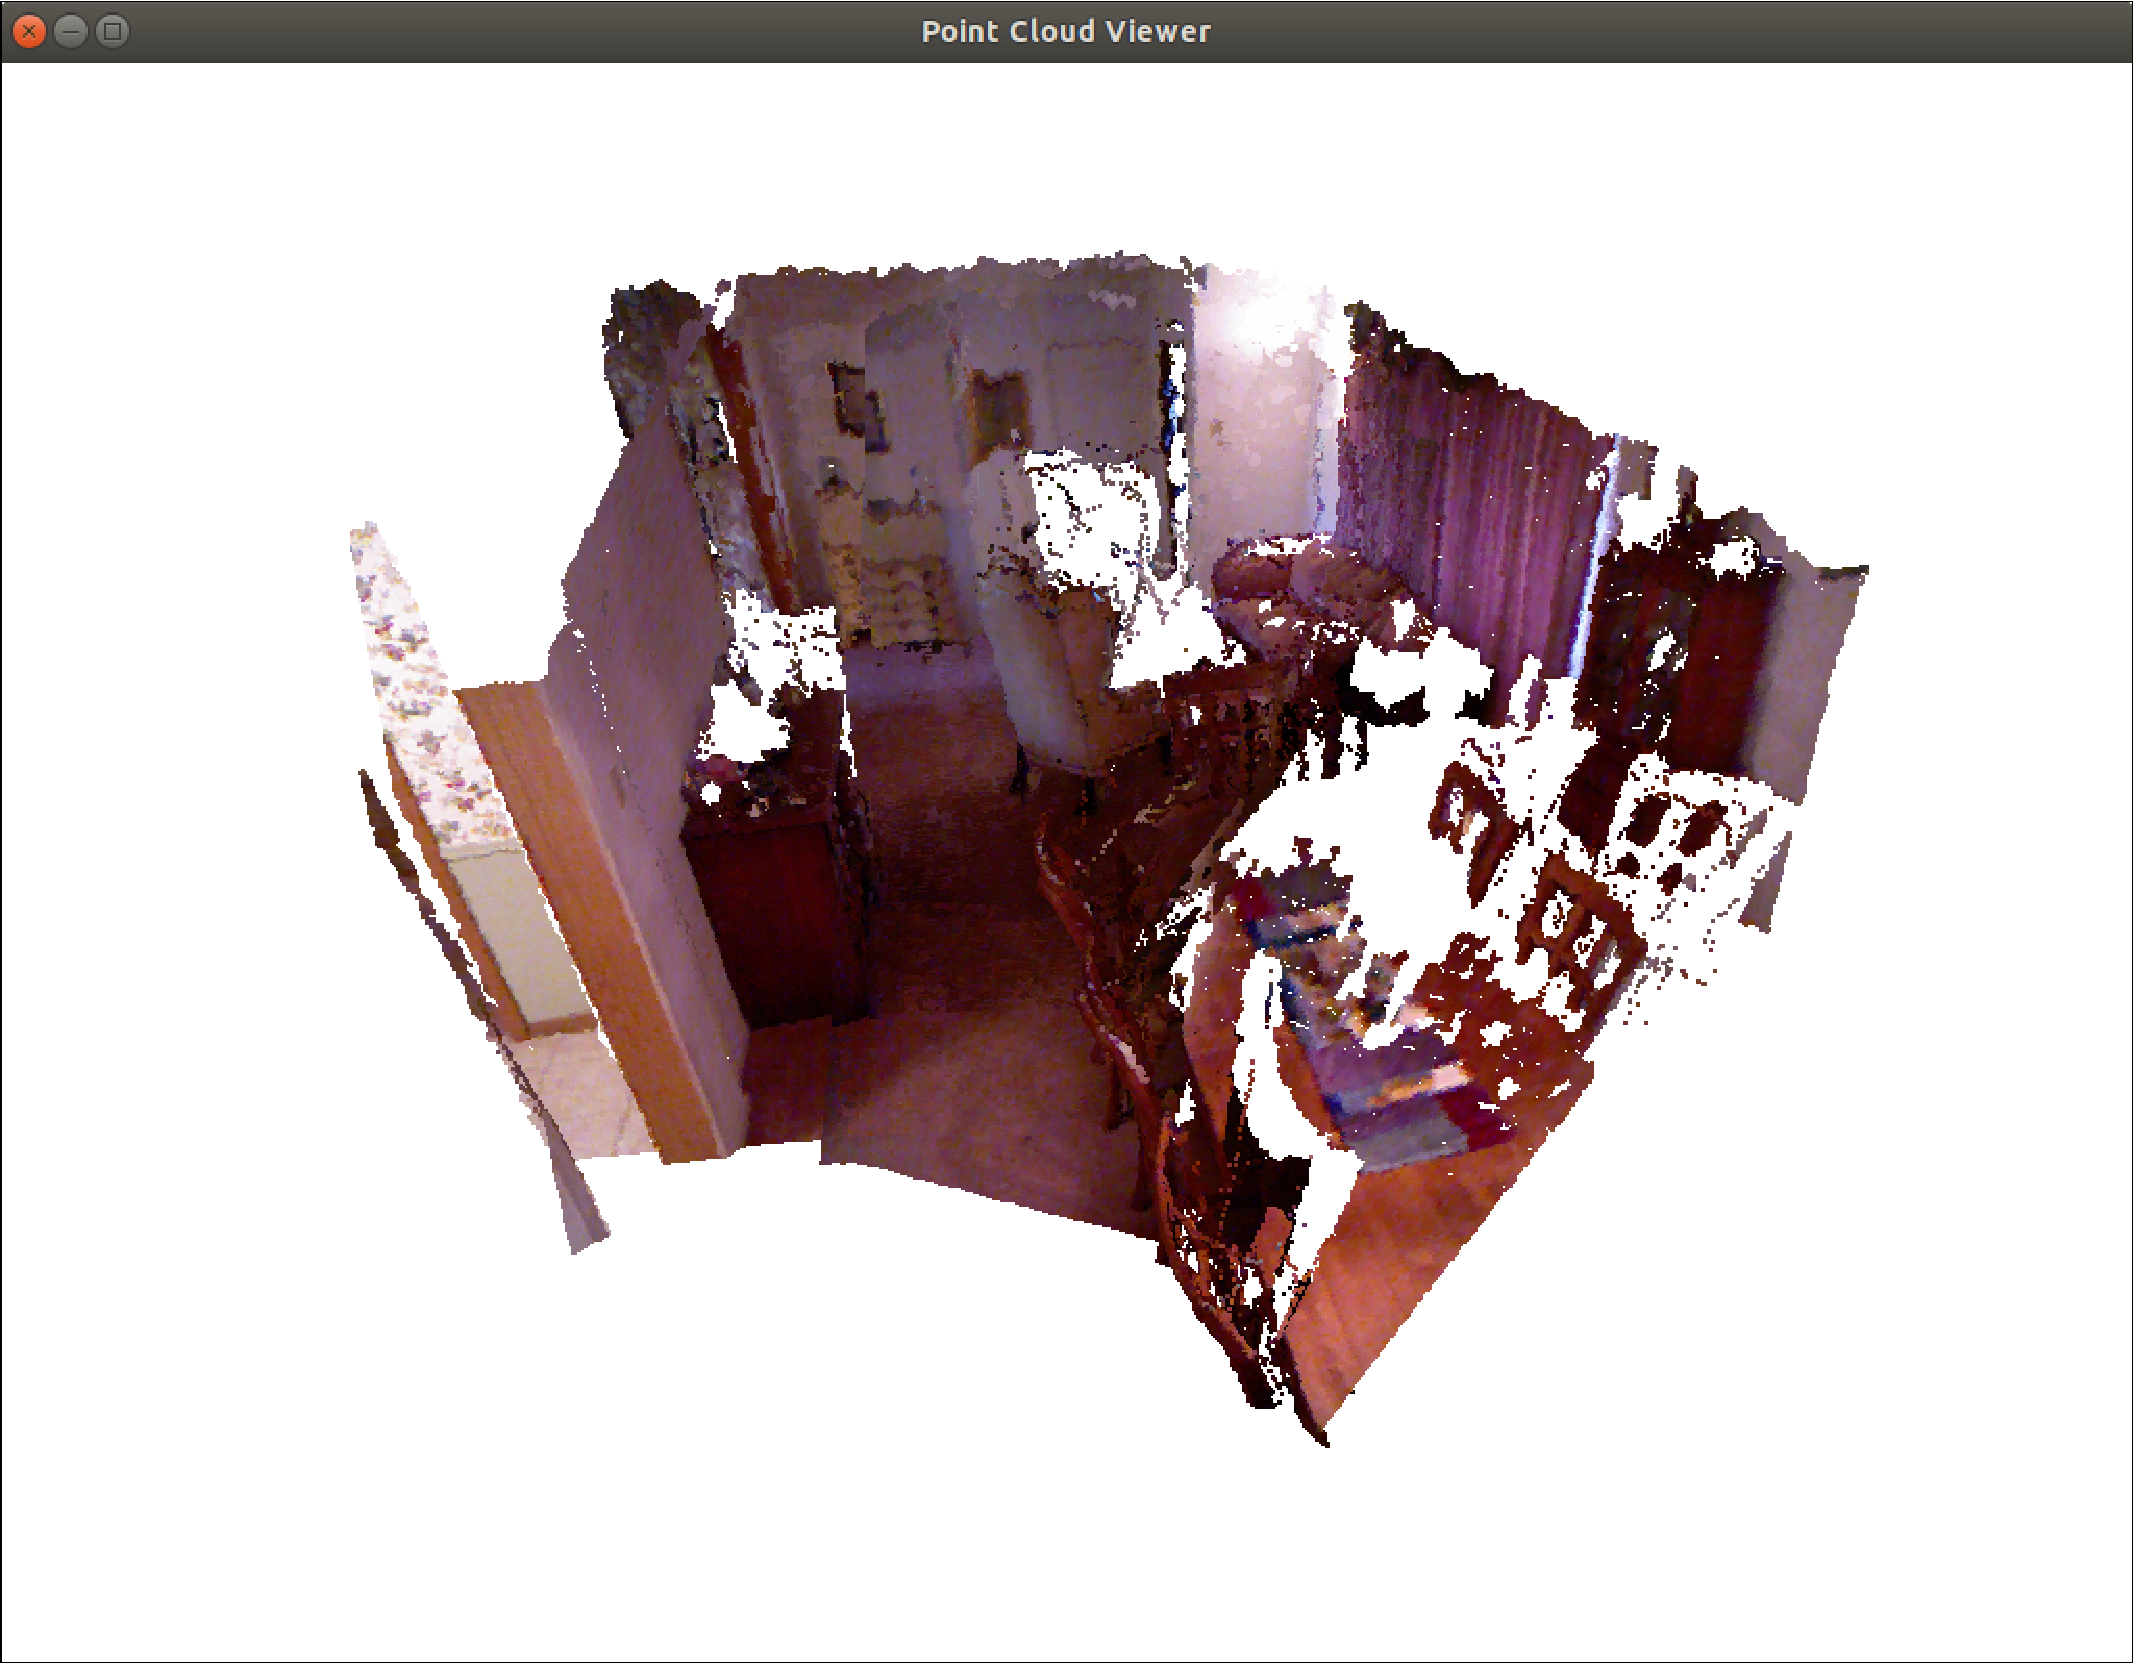
\includegraphics[width=1.0\textwidth]{chapter05/resources/cameraModel/pointcloud.pdf}
	\caption{View the stitched point cloud map. }
	\label{fig:pointcloudmapping}
\end{figure}

Through these examples, we demonstrate some common monocular, binocular, and depth camera algorithms in computer vision. I hope that readers can actually understand the meaning of the internal and external parameters and distortion parameters of the camera through these simple examples.